\documentclass[11pt,a4paper]{article}

\usepackage[T1]{fontenc}
\usepackage[utf8]{inputenc}
\usepackage[margin=17mm]{geometry}
\usepackage{helvet}
\renewcommand{\familydefault}{\sfdefault}

\usepackage{xcolor}
\usepackage{booktabs}
\usepackage{graphicx}
\usepackage{longtable}
\usepackage{array}
\usepackage{enumitem}
\usepackage{textcomp}
\usepackage{hyperref}
\usepackage{tcolorbox}
\usepackage{parskip}
\usepackage{titlesec}
\usepackage{fancyhdr}
\usepackage{lastpage}
\usepackage{attachfile2}

% ── Color Palette (matching Project Charter) ──────────────────────────
\definecolor{ISAAIBlue}{HTML}{00335b}
\definecolor{ISAAIBlueLight}{HTML}{00508f}
\definecolor{ISAAIGreen}{HTML}{007a33}
\definecolor{ISAAIRed}{HTML}{d11241}
\definecolor{ISAAIMuted}{HTML}{666666}
\definecolor{ISAAIBorder}{HTML}{d1d5db}
\definecolor{ISAAIWarnBg}{HTML}{fffbeb}
\definecolor{ISAAIWarnText}{HTML}{92400e}

\hypersetup{
  colorlinks=true,
  linkcolor=ISAAIBlueLight,
  urlcolor=ISAAIBlueLight,
  pdftitle={ISAAI -- Automatic Report Documentation},
  pdfauthor={Christina Malki, Altay Hennig},
}

% ── Section styling ───────────────────────────────────────────────────
\titleformat{\section}
  {\color{ISAAIBlue}\Large\bfseries}
  {\thesection.}{0.5em}{}
\titleformat{\subsection}
  {\color{ISAAIBlue}\large\bfseries}
  {\thesubsection}{0.5em}{}

% ── Header / Footer ──────────────────────────────────────────────────
\pagestyle{fancy}
\fancyhf{}
\fancyhead[L]{\small\color{ISAAIMuted}ISAAI -- Automatic Report Documentation}
\fancyhead[R]{\small\color{ISAAIMuted}Summer Semester 2026}
\fancyfoot[C]{\small\color{ISAAIMuted}\thepage\ / \pageref{LastPage}}
\renewcommand{\headrulewidth}{0.4pt}
\renewcommand{\footrulewidth}{0pt}

% ── Meta-tag command ─────────────────────────────────────────────────
\newcommand{\metatag}[1]{%
  \tcbox[
    on line,
    arc=2pt,
    boxrule=0.4pt,
    colback=gray!10,
    colframe=ISAAIBorder,
    left=3pt,right=3pt,top=1pt,bottom=1pt
  ]{\scriptsize\bfseries #1}%
}

\begin{document}

% ══════════════════════════════════════════════════════════════════════
%  TITLE PAGE
% ══════════════════════════════════════════════════════════════════════

\thispagestyle{empty}

\begin{center}
  \vspace*{3cm}

  {\color{ISAAIBlue}\Huge\bfseries ISAAI}\\[0.3em]
  {\color{ISAAIBlue}\LARGE Automatic Report Documentation}\\[1.5em]

  {\large Final Report -- Summer Semester 2026}\\[0.5em]
  {\small\color{ISAAIMuted} Frankfurt University of Applied Sciences -- FB2}\\[3em]

 
  \begin{tabular}{@{}rl@{}}
    \textbf{Module:}      & ISA (Information Systems Architecture) \\[0.3em]
    \textbf{University:}  & Frankfurt University of Applied Sciences --- Faculty~2 \\[0.3em]
    \textbf{Semester:}    & Summer Semester 2026 \\[0.3em]
    \textbf{Project Team:} & Altay Hennig (1483613) \\
                           & Christina Malki (1574803) \\
                           & Sarah Bullinger (1577846) \\[0.3em]
    \textbf{E-Mail:}      & \href{mailto:altay.hennig@stud.fra-uas.de}{altay.hennig@stud.fra-uas.de} \\
                           & \href{mailto:christina.malki@stud.fra-uas.de}{christina.malki@stud.fra-uas.de} \\
                           & \href{mailto:sarah.bullinger@stud.fra-uas.de}{sarah.bullinger@stud.fra-uas.de} \\[0.3em]
    \textbf{Examiner:}   & Mr.\ Dominik Dietrich \\[0.3em]
    \textbf{Date:}        & Juli 31, 2026 \\
  \end{tabular}

  \vfill
  {\small\color{ISAAIMuted}
    Repository:
    \url{https://github.com/pollo60/-ISAAI-Automatic-Report-Documentation}}

\end{center}

\newpage

% ══════════════════════════════════════════════════════════════════════
%  TABLE OF CONTENTS
% ══════════════════════════════════════════════════════════════════════

\tableofcontents
\newpage


% ══════════════════════════════════════════════════════════════════════
%  1. INTRODUCTION
% ══════════════════════════════════════════════════════════════════════

\section{Introduction}

The ISAAI project --- short for \emph{Information Systems Architecture and Integration} --- was carried out during the summer semester of 2026 at the Frankfurt University of Applied Sciences. It spans two complementary modules: \emph{Information Systems Architecture (ISA)} and \emph{Architecture and Integration (A+I)}, both supervised by Prof.~Dr.~Dominik Dietrich in Faculty~2. The central motivation behind the project is the automation of a daily, compliance-critical business process that, in its current form, consumes significant operational effort and is prone to human error.

\subsection{Project Context}

In the day-to-day operations of a financial service provider, two types of structured reports arrive every morning via e-mail. \textbf{Report Type~A} captures the previous business day's trade-level details in a daily snapshot, while \textbf{Report Type~B} provides a month-to-date cumulative summary of trader activity. Both reports are delivered as XML files packaged inside ZIP archives and contain compliance-relevant markers --- so-called \emph{DayViol} and \emph{MonthViol} flags --- that indicate whether trading thresholds have been breached.

Until now, this entire workflow has been performed manually: an employee opens the incoming e-mail, extracts the ZIP archive, imports the XML data into a spreadsheet, visually inspects the violation markers, creates evidence documents, archives them, and escalates any issues to a supervisor. The whole cycle takes between 30 and 40 minutes each day --- time that could be spent on higher-value analytical tasks instead.

\subsection{Dual Module Approach}

Because the project serves two university modules simultaneously, the work is organized along two tracks that reinforce each other. The A+I track focuses on the operative process automation itself: building the end-to-end pipeline that ingests Report~A and Report~B, evaluates compliance rules, generates evidence files, and manages exception governance. The ISA track, on the other hand, contributes the enterprise architecture perspective --- ArchiMate modeling across three transformation stages, BPMN process models, and a parallel university deliverable covering invoice analysis with chart automation.

\begin{table}[ht]
\centering
\caption{Module Comparison}
\begin{tabular}{@{}p{0.12\textwidth}p{0.38\textwidth}p{0.38\textwidth}@{}}
\toprule
\textbf{Module} & \textbf{Focus} & \textbf{Technology} \\
\midrule
A+I & Enterprise Architecture, ArchiMate Modeling, Invoice and Chart Automation & ArchiMate, Power Automate, PowerPoint \\
ISA & Operative Process Automation, XML Validation, Exception Governance, GOAL BPMN & Power Automate, PowerPoint, Camunda Modeler \\
\bottomrule
\end{tabular}
\end{table}

This dual-track structure ensures that the project is both architecturally grounded and practically relevant. The ArchiMate diagrams provide the strategic ``big picture,'' while the Power Automate implementation delivers a working, deployable solution.

\subsection{Project Goal}

The overarching goal of the project can be stated concisely: \emph{eliminate the 30--40 minutes of daily manual effort while preserving full auditability and human oversight for exceptions}. More precisely, the system should automatically detect incoming report e-mails, extract and parse the XML content, evaluate the compliance rules in parallel for both report types, generate professionally formatted evidence documents, and store everything in a traceable audit trail on SharePoint. Human intervention should be required only when an actual rule violation is detected --- the classic \emph{human-in-the-loop} pattern.

To ensure this goal is concrete and measurable, it was formulated according to the SMART framework:

\begin{table}[ht]
\centering
\caption{SMART Goal Framework}
\begin{tabular}{@{}ccccc@{}}
\toprule
\textbf{Specific} & \textbf{Measurable} & \textbf{Achievable} & \textbf{Relevant} & \textbf{Time-bound} \\
\midrule
\begin{minipage}[t]{0.16\textwidth}\small Report~A/B XML Pipeline + parallel ISA Invoice Pipeline\end{minipage} &
\begin{minipage}[t]{0.16\textwidth}\small End-to-End Automation for the standard path; Exceptions measurable\end{minipage} &
\begin{minipage}[t]{0.16\textwidth}\small GitHub CI/CD, Mock APIs, existing BPMN/ArchiMate models\end{minipage} &
\begin{minipage}[t]{0.16\textwidth}\small White-box interfaces; Audit Trail; 30--40 min/day time savings\end{minipage} &
\begin{minipage}[t]{0.16\textwidth}\small Deadline June~30, 2026\end{minipage} \\
\bottomrule
\end{tabular}
\end{table}

\subsection{Project Organization}

The project team consists of three core members, each with clearly defined responsibilities:

\begin{table}[ht]
\centering
\caption{Project Organization}
\begin{tabular}{@{}p{0.35\textwidth}p{0.55\textwidth}@{}}
\toprule
\textbf{Role} & \textbf{Person / Unit} \\
\midrule
Sponsor and Academic Lead & Dominik Dietrich --- FRA UAS / FB2 \\
Architecture and Software Engineering & Christina Malki, Altay Hennig --- Modules ISA and A+I \\
Operative Owner & Sarah Bullinger --- Project Management Operations \\
\bottomrule
\end{tabular}
\end{table}


% ══════════════════════════════════════════════════════════════════════
%  2. MANAGEMENT SUMMARY
% ══════════════════════════════════════════════════════════════════════

\section{Management Summary}

\subsection{Solution Overview}

The ISAAI system replaces the entire manual report processing workflow with a fully automated \textbf{Microsoft Power Automate Cloud Flow}. When an e-mail with the subject ``Financial Report'' arrives in the designated mailbox, the flow is triggered automatically. It extracts the ZIP attachment, unpacks both XML report files, and processes them in parallel through dedicated parsing and validation branches.

For each report type, the system applies XPath-based rule evaluation to detect violation markers. If both reports pass without violations, the flow generates professionally styled XLSX evidence documents, saves them to a SharePoint Document Library, drafts a summary e-mail for the relevant stakeholders, sends it, and archives a copy of the sent message. If a rule violation is detected, the flow follows the exception governance path: it generates an exception alert that is escalated to the Operations Supervisor, who then reviews the violation and executes any necessary governance actions.

Throughout this process, every step is logged in a SharePoint List that serves as the operational database. This creates a seamless audit trail satisfying both internal compliance requirements and the traceability demands of external audits.

\subsection{Key Result}

The automation eliminates the entire daily manual effort of 30 to 40 minutes while ensuring full auditability. Human control is preserved where it matters most --- for exception handling and governance sign-off --- but the routine, error-prone manual steps are completely removed from the process.


% ══════════════════════════════════════════════════════════════════════
%  3. PROBLEM DESCRIPTION
% ══════════════════════════════════════════════════════════════════════

\section{Problem Description}

\subsection{As-Is State (CURRENT State)}

In the current state, daily financial reports are processed entirely by hand. The workflow begins when an employee receives a daily e-mail containing a ZIP archive with two XML report files. The employee manually unpacks the archive, opens the XML files, and imports the data into a spreadsheet application. There, violation markers and threshold values are checked visually --- a task that requires concentration and domain knowledge, yet is highly repetitive and offers little room for value-adding analysis.

Once the check is complete, the employee creates evidence documents to record the results, formats them according to internal standards, and files them in the company's document management system. If any violations are found, they must be flagged and escalated to a supervisor, who reviews the case and decides on appropriate governance actions. Finally, a summary is distributed to the relevant stakeholders. This entire cycle --- extraction, validation, documentation, archiving, and distribution --- takes approximately 30 to 40 minutes every business day.

The corresponding BPMN process model for the CURRENT state is available in the project repository as a \texttt{.bpmn} file, documenting the manual flow in detail.

\subsection{Identified Weaknesses}

Several structural weaknesses make this manual process particularly problematic. The most obvious is the \textbf{time consumption}: dedicating 30 to 40 minutes of skilled labor every day to a routine task is an inefficient use of resources. Beyond time, the process involves a significant \textbf{media break} --- employees must switch between the e-mail client, a file explorer, a spreadsheet application, and the document management system, each transition creating opportunities for errors and information loss.

There is also a \textbf{lack of system enforcement}: no automated mechanism ensures that the upload-to-sign-off workflow is followed correctly every time. This creates compliance risk and makes it difficult to trace exactly what happened during any given processing run. Finally, the reliance on \textbf{human judgment} for routine checks introduces the risk of inconsistent outputs, forgotten steps, and quality defects that could surface during audits.

\begin{table}[ht]
\centering
\caption{Identified Weaknesses in As-Is Process}
\begin{tabular}{@{}p{0.22\textwidth}p{0.35\textwidth}p{0.33\textwidth}@{}}
\toprule
\textbf{Weakness} & \textbf{Description} & \textbf{Impact} \\
\midrule
Time Consuming & 30--40 minutes of daily manual effort & Loss of productivity, resource binding \\
Media Break & Switching between Collaboration Storage and Document Repository & Susceptibility to errors, loss of information \\
Lack of System Enforcement & No system-supported upload-to-sign-off process & Compliance risk, lack of traceability \\
Human Errors & Incorrect fields, inconsistent outputs, forgotten steps & Quality defects, audit risks \\
\bottomrule
\end{tabular}
\end{table}

\subsection{Risk and Control Gap}

Manual processing multiplies traceability gaps and increases the risk of unauthorized changes or overlooked violations. Without automation, there is no standardized audit trail --- each processing run depends on the individual employee's diligence and familiarity with the procedure. This lack of standardization exacerbates compliance risk and makes it difficult to demonstrate regulatory conformity during audits.

\subsection{Report Types}

The two report types differ in their temporal scope and analytical purpose, but share the same delivery mechanism and compliance-relevant structure:

\begin{table}[ht]
\centering
\caption{Report Types A and B Characteristics}
\begin{tabular}{@{}p{0.20\textwidth}p{0.35\textwidth}p{0.35\textwidth}@{}}
\toprule
\textbf{Attribute} & \textbf{Report Type A (Daily)} & \textbf{Report Type B (Monthly)} \\
\midrule
Coverage Period & Previous business day (Trade-Level Detail) & Month-to-Date cumulative trader summary \\
Delivery Frequency & Daily, at the agreed processing time & Daily, together with Report Type~A \\
Violation Marker & DayViol & MonthViol \\
Purpose & Detection of same-day trade exceptions & Tracking monthly cumulative trader breach trends \\
\bottomrule
\end{tabular}
\end{table}


% ══════════════════════════════════════════════════════════════════════
%  4. SOLUTION DESIGN
% ══════════════════════════════════════════════════════════════════════

\section{Solution Design}

\subsection{Architecture Evolution: CURRENT $\rightarrow$ GOAL}

The project follows a three-stage architecture evolution model that is common in enterprise architecture practice. The \textbf{CURRENT} state documents the manual as-is process. The \textbf{VISION} state represents the ideal fully automated target, including integration with the company's internal Document Management System via UI scraping or RPA. The \textbf{GOAL} state is the pragmatically scoped, actually implemented solution --- it delivers full automation of the core workflow while deliberately excluding the DMS integration, which proved impractical within the project constraints.

\begin{figure}[ht]
\centering
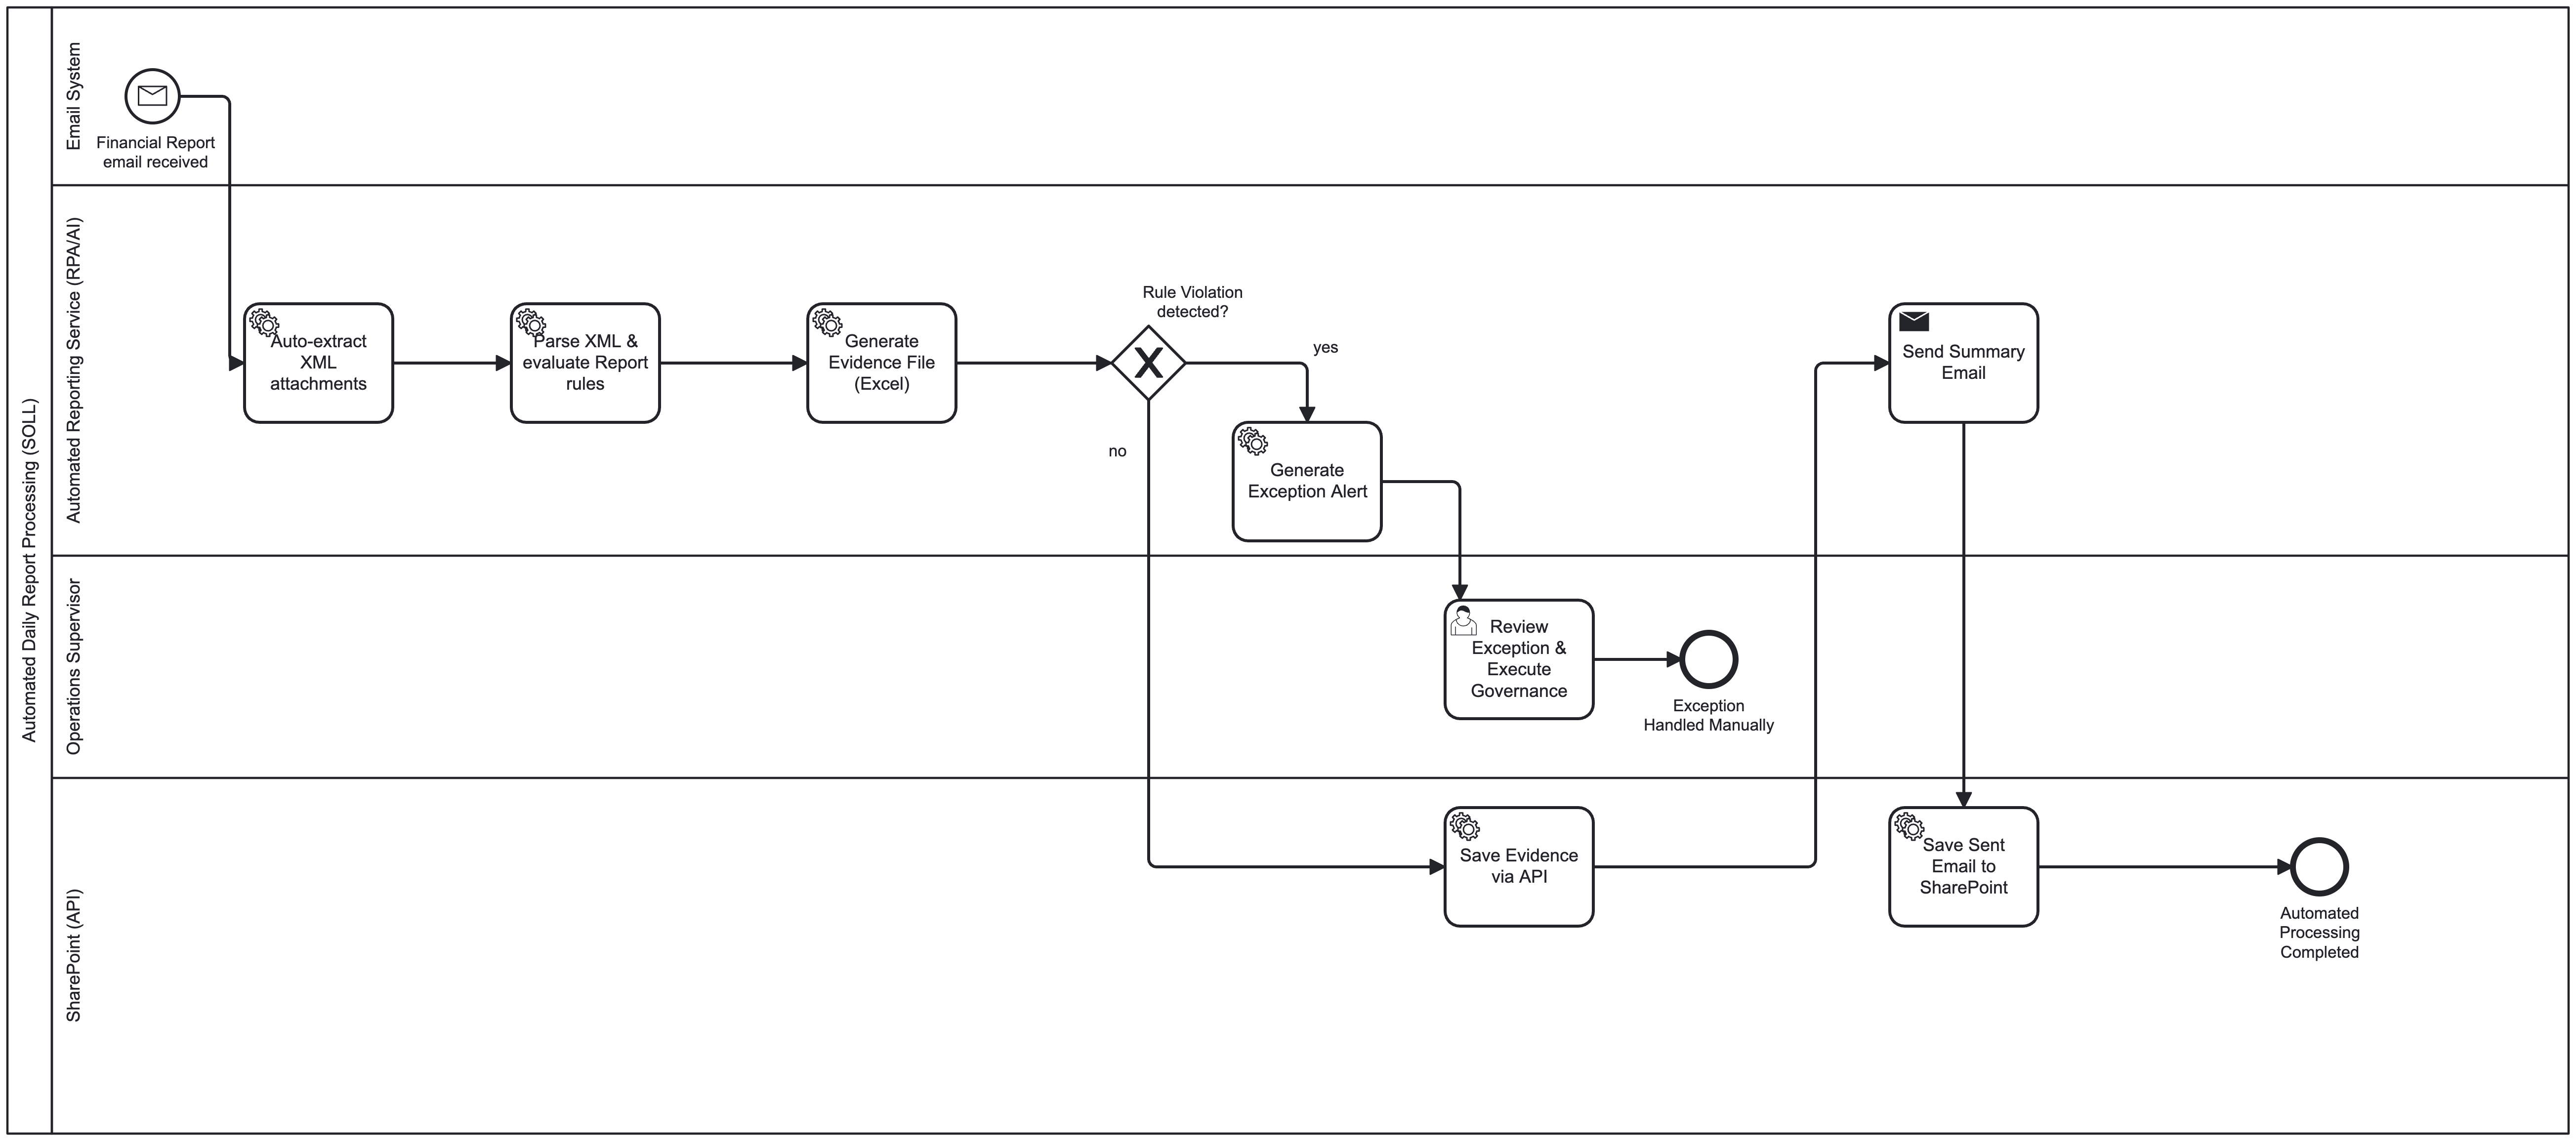
\includegraphics[width=\textwidth]{strategic_goal_bpmn.png}
\caption{Strategic BPMN GOAL Process \textattachfile[mimetype=application/xml, description={Strategic GOAL BPMN Process Model}]{strategic_goal.bpmn}{[\texttt{📎 Download .bpmn}]}}
\end{figure}

This three-tier approach is documented in both ArchiMate~3.1 models (available as \texttt{.archimate} files) and BPMN~2.0 process models (available as \texttt{.bpmn} files) in the project repository. The models trace the transformation path from manual operations to automated processing, making every architectural decision transparent and traceable.

The project utilizes already realized automation capabilities provided by Microsoft as part of their Office~365 suite. Rather than building custom infrastructure from scratch, the solution leverages Power Automate's native connectors for Exchange, SharePoint, and XML processing. This approach minimizes development effort while maximizing reliability and maintainability.

\subsection{GOAL (Realized State)}

The GOAL state represents what was actually built and deployed. It is a fully functional Microsoft Power Automate Cloud Flow that handles the complete report processing pipeline --- from e-mail detection through XML parsing, rule evaluation, evidence generation, and SharePoint archiving to stakeholder notification.

The DMS integration that was envisioned in the VISION state was deliberately excluded from the GOAL scope. SharePoint serves as the sole Evidence Repository, which is both simpler and more maintainable than the originally planned DMS integration via UI scraping. This pragmatic scope reduction is a conscious architectural decision, not a compromise in functionality: SharePoint fully satisfies the requirements for traceable evidence storage and audit trail documentation.

\subsection{Power Automate Flow --- Technical Architecture}

The flow \emph{ISAAI -- Daily Report Processing} is structured into six sequential phases and is available as an importable Power Automate package in the repository under \texttt{src/flow/ISAAI-Daily\-Report\-Processing\_20260625165442.zip}. The six phases cover trigger detection, ZIP extraction, parallel XML parsing, rule-based validation, evidence generation with SharePoint archiving, and summary e-mail distribution. Each phase is designed to be independently testable and produces traceable outputs that are logged in the SharePoint List.

\subsection{Technology Stack}

The solution is built on a carefully chosen set of technologies that balance capability with accessibility:

\begin{table}[ht]
\centering
\caption{Technology Stack}
\begin{tabular}{@{}p{0.30\textwidth}p{0.60\textwidth}@{}}
\toprule
\textbf{Component} & \textbf{Technology} \\
\midrule
Automation & Microsoft Power Automate (Cloud Flow) \\
Data Storage & SharePoint Online (Lists + Document Library) \\
Evidence Format & XLSX (Excel) \\
Architecture Modeling & ArchiMate 3.1 (Archi) \\
Process Modeling & BPMN 2.0 (Camunda Modeler) \\
Local Simulation & Python 3, openpyxl, python-pptx \\
Version Control & Git / GitHub \\
Artificial Intelligence & Gemini, Claude, Antigravity, CursorAI \\
\bottomrule
\end{tabular}
\end{table}

The choice of Power Automate as the automation platform was driven by the organization's existing Microsoft~365 licensing. Using a low-code platform rather than custom code significantly reduces the maintenance burden and makes the solution accessible to non-developers in the operations team. Python was used for local simulation and testing, generating reproducible mock data for 30 test runs to validate the logic before deployment.


% ══════════════════════════════════════════════════════════════════════
%  5. CHALLENGES
% ══════════════════════════════════════════════════════════════════════

\section{Challenges}

\subsection{Power Automate}

Working with Microsoft Power Automate presented several practical challenges that are worth documenting for future projects. The platform's AI-assisted flow generation (Microsoft Copilot) was unable to generate or import complex branching flows reliably. Specifically, the parallel processing of two report types with conditional error handling and exception governance exceeded the complexity that Copilot could handle in a single generation step. As a result, the entire flow had to be designed and built manually in the Power Automate Designer, step by step.

A detailed guide documenting the manual build process was created and stored in the repository under \texttt{docs/guides/SHAREPOINT\_FLOW\_GUIDE.md}. This guide serves both as internal documentation and as a reference for anyone who needs to modify or extend the flow in the future.

\subsection{DMS Integration (Out of Scope)}

The original VISION called for full integration with the company's internal Document Management System, including UI scraping and RPA-based automation to upload evidence documents and obtain sign-off approvals. During the analysis phase, however, several factors made this integration impractical for the project scope.

First, UI scraping is inherently fragile: any change to the DMS user interface would break the automation, requiring constant maintenance. Second, no stable API to the DMS was available, which meant that all interaction would have had to go through the graphical user interface --- a fundamentally unreliable approach for production use. Third, and most importantly, SharePoint already provides all the functionality needed for evidence storage and audit trail documentation.

The decision to exclude DMS integration was therefore not a failure to meet requirements, but a deliberate, well-reasoned architectural decision that prioritizes reliability and maintainability over theoretical completeness. This kind of pragmatic scope management is a valuable skill in both academic and corporate settings.


% ══════════════════════════════════════════════════════════════════════
%  6. LESSONS LEARNED AND FINDINGS
% ══════════════════════════════════════════════════════════════════════

\section{Lessons Learned and Findings}

\subsection{Architecture and Modeling}

One of the most significant insights from this project concerns the role of ArchiMate modeling in practice. While the three-tier architecture evolution (CURRENT~$\rightarrow$~VISION~$\rightarrow$~GOAL) was conceived primarily as a university deliverable, the models proved to be unexpectedly valuable as a communication tool.

When presenting the project to stakeholders, the ArchiMate diagrams provided a clear, visual way to explain the transformation path from manual to automated processing. Each layer of the model --- from the business motivation through the application architecture to the technology stack --- told a coherent story about why the project exists, what it changes, and how it delivers value. This experience suggests that in professional practice, architecture models are most effective when they are used as communication instruments rather than purely technical documentation.

The project also revealed an interesting distinction between ArchiMate usage for internal strategy discussions versus delivery-oriented communication. The same model can be ``sliced'' differently depending on the audience: a governance-focused view emphasizes compliance controls and exception paths, while a technology-focused view highlights integration points and data flows. This compartmentalization approach can significantly increase the efficiency and clarity of stakeholder communications.

\subsection{Technology and Automation}

Power Automate proved to be well-suited for the defined use case. The combination of an e-mail trigger, ZIP extraction, XML parsing, rule-based validation, and SharePoint storage fits naturally into Power Automate's connector-based architecture. Each of these operations corresponds to a native connector or a well-documented action, which minimized the amount of custom logic needed.

However, the project also demonstrated the limitations of low-code platforms. Complex branching logic --- particularly parallel processing with error handling on multiple branches --- pushes Power Automate to the edge of its design paradigm. The visual flow designer becomes unwieldy at a certain level of complexity, and debugging parallel branches requires careful attention to variable scoping and error propagation. For future projects with even more complex logic, a hybrid approach combining Power Automate for orchestration with Azure Functions for complex processing steps might be worth considering.


% ══════════════════════════════════════════════════════════════════════
%  7. OUTCOME AND CONCLUSION
% ══════════════════════════════════════════════════════════════════════

\section{Outcome and Conclusion}

\subsection{Project Result}

The ISAAI project achieved all of its defined goals within the planned timeline. The following table provides a concise overview of each goal and its completion status:

\begin{table}[ht]
\centering
\caption{Project Results Overview}
\begin{tabular}{@{}p{0.28\textwidth}cp{0.50\textwidth}@{}}
\toprule
\textbf{Goal} & \textbf{Status} & \textbf{Description} \\
\midrule
Full automation of the standard path & Achieved & E-Mail, ZIP, XML, Validation, Evidence, SharePoint, Notification \\
Exception Governance & Achieved & Human-in-the-loop for violations with supervisor escalation \\
Audit Trail & Achieved & Seamless documentation in SharePoint List + Document Library \\
ArchiMate Modeling (3 stages) & Achieved & CURRENT, VISION, GOAL each as ArchiMate models (\texttt{.archimate}) \\
BPMN Process Modeling (3 stages) & Achieved & CURRENT, VISION, GOAL each as BPMN diagrams (\texttt{.bpmn}) \\
Power Automate Flow & Achieved & Importable flow package in the repository \\
Local Simulation & Achieved & 30 reproducible test runs with Python scripts \\
ISA Module (parallel) & Achieved & Invoice receipt, JSON/CSV, Chart Automation \\
Presentation Material & Achieved & Consolidated Findings Deck + Module Presentations \\
\bottomrule
\end{tabular}
\end{table}

\subsection{Quantitative Benefits}

Beyond the qualitative improvements in process reliability and auditability, the project also delivers measurable economic benefits. A cost-benefit analysis based on the Function Point and COCOMO estimation methods puts the total implementation effort at approximately 323 working hours. Including allowances for project coordination, change management, training, and a reasonable contingency buffer, the estimated total cost comes to \textbf{9,656.40\,\texteuro{}}.

This investment pays for itself through the daily elimination of 30 to 40 minutes of manual labor. Over the course of a year, this amounts to roughly 130 to 170 hours of freed-up capacity --- operational time that can be redirected toward higher-value activities such as analytical review, process improvement, and strategic planning.

\subsection{Conclusion}

The ISAAI project demonstrates convincingly how the combination of enterprise architecture methodology (ArchiMate, BPMN) and low-code automation (Power Automate, SharePoint) can completely transform an operational process. The systematic documentation of the transformation path across three architecture stages --- CURRENT, VISION, and GOAL --- ensures that every decision is traceable and that the solution remains comprehensible and maintainable over time.

The deliberate scope reduction from VISION to GOAL, specifically the exclusion of DMS integration, also illustrates an important practical lesson: pragmatic architecture decisions are just as important in a university project as they are in corporate practice. It is better to deliver a complete, reliable solution within a well-defined scope than to attempt a more ambitious target that cannot be fully realized. The SharePoint-based solution meets all functional requirements while providing a solid, extensible foundation for future enhancements --- including, potentially, the DMS integration that was deferred from the original VISION.


% ══════════════════════════════════════════════════════════════════════
%  8. MAGIC CHARTS
% ══════════════════════════════════════════════════════════════════════

\section{Magic Charts}

\subsection{Concept}

A distinctive feature of the ISAAI project is the \emph{Magic Charts} module --- a collection of Python scripts that automate the creation of visualizations and presentations from the processed report data. The underlying idea is straightforward: since the evidence files produced by the Power Automate Flow are stored in structured, machine-readable formats (XLSX), they can serve as input for automated chart generation and presentation building. This transforms raw compliance data into professional, meaningful visual artifacts without any manual formatting effort.

\subsection{Implemented Scripts}

The Magic Charts module comprises five interconnected scripts, each serving a specific purpose in the data-to-presentation pipeline:

\begingroup\sloppy
\textbf{Test Data Generation} (\texttt{simulate\_runs.py}) produces reproducible mock XML and ZIP test data for 30 simulated business days. This script was essential during development, as it allowed the team to test the entire pipeline end-to-end without depending on live report data.

\textbf{Local Flow Processing} (\texttt{local\_flow\_processor.py}) simulates the full Power Automate Flow offline and generates professionally styled evidence files. This local simulation capability was invaluable for development and debugging, enabling rapid iteration without deploying to the cloud environment.

\textbf{Consolidated Findings Presentation} (\texttt{generate\_findings\_presentation.py}) aggregates the results from all test runs into a single, coherent findings presentation that provides a high-level overview of compliance trends and exception patterns.

\textbf{Boardroom Deck} (\texttt{build\_boardroom\_deck.py}) generates a management-ready presentation with executive-level visualizations and key metrics, suitable for governance meetings and stakeholder briefings.

\textbf{Demo Flow} (\texttt{demo\_flow.py}) provides an interactive demonstration mode that walks through a single processing run with visual output, making it easy to showcase the system's capabilities to non-technical audiences.
\endgroup


% ══════════════════════════════════════════════════════════════════════
%  9. SOURCES
% ══════════════════════════════════════════════════════════════════════

\begingroup\sloppy
\section{Sources}

\subsection{Architecture and Modeling}

\begin{enumerate}[leftmargin=*, nosep]
  \item ArchiMate 3.1 Specification. The Open Group. \url{https://pubs.opengroup.org/architecture/archimate3-doc/}
  \item Archi --- ArchiMate Modelling Tool. \url{https://www.archimatetool.com/}
  \item BPMN 2.0 Specification. Object Management Group (OMG). \url{https://www.omg.org/spec/BPMN/2.0/}
  \item Camunda BPMN Modeler. Camunda Services GmbH. \url{https://camunda.com/}
\end{enumerate}

\subsection{Compliance and Governance}

\begin{enumerate}[leftmargin=*, nosep]
  \item EU AI Act --- Regulation (EU) 2024/1689. European Parliament and Council. \url{https://eur-lex.europa.eu/eli/reg/2024/1689/oj}
  \item General Data Protection Regulation (GDPR) --- Regulation (EU) 2016/679. European Parliament and Council. \url{https://eur-lex.europa.eu/eli/reg/2016/679/oj}
\end{enumerate}

\subsection{Development Tools}

\begin{enumerate}[leftmargin=*, nosep]
  \item Python 3 Documentation. Python Software Foundation. \url{https://docs.python.org/3/}
  \item openpyxl --- A Python library to read/write Excel 2010 xlsx/xlsm/xltx/xltm files. \url{https://openpyxl.readthedocs.io/}
  \item python-pptx --- Python library for creating PowerPoint files. \url{https://python-pptx.readthedocs.io/}
  \item GitHub --- Collaborative Development Platform. \url{https://github.com/}
\end{enumerate}

\subsection{Project Resources}

\begin{enumerate}[leftmargin=*, nosep]
  \item ISAAI GitHub Repository. All attachments can be accessed via the following repository: \url{https://github.com/pollo60/-ISAAI-Automatic-Report-Documentation}
  \item SharePoint Site --- ISAAI Daily Report Processing. \url{https://studfrauasde.sharepoint.com/sites/ISAAIDailyReportProcessing}
\end{enumerate}
\endgroup

\vfill
\hrule
\small\color{ISAAIMuted}
Project ownership: Prof.\ Dr.\ Dominik Dietrich (sponsor) \textbar\
Christina Malki, Altay Hennig (engineering) \textbar\
Sarah Bullinger (operations)

\end{document}
